\chapter{Conversations for On-Trip Voice Guidance}
While nudging drivers to choose an unselfish route can be achieved through theory-based design as shown in Chapter 5, we are only halfway into achieving our goals. Chapter 4 extends empirical evidence from GPS tracks and recorded actual trips that show that drivers do not always prefer the fastest routes \cite{Quercia2014, Zhu2015DoPrinciple,Tang2016AnalyzingData,Fujino2018DetectingTracks,Brown2012TheGPS,Samson:2019:EFI:3290605.3300601} and shows that after choosing a route to follow, drivers are still likely to deviate because of \emph{normal, natural troubles} that they experience with GPS devices \cite{Brown2012TheGPS}, road unfamiliarity, and perceived impracticality and driving unsuitability \cite{Samson:2019:EFI:3290605.3300601}. Thus, it is equally important to rethink how voice guidance can be improved to effectively support driver during a trip. Because despite being offered in GPS devices since the 1990s, there are still gaps in current systems and applications that fail to consider the changing contexts and preferences which shapes the realization of a navigation task. 

Echoing Brown \& Laurier \cite{Brown2012TheGPS} in their call to not think of drivers as docile actors and to focus more on helping them make \textit{instructed actions} when designing voice guidance, our design goal is to support a driver's ability to interpret and analyze new route guidance and information in order to help them make better navigation decisions. Specifically, we focus on exploring how to provide ample route information and alternative suggestions for some turns during a trip, providing them agency.

Essentially, navigation is a social activity among drivers and navigators \cite{Forlizzi2010WhereTurn, Matsumura2014WhatDriving}. And despite our growing reliance on modern navigation systems, we still perform better in terms of navigation and route learning when we are with an active collaborative partner in the task \cite{Antrobus2017Driver-PassengerSystems, antrobus_large_burnett_hare_2019, Brown2012TheGPS}. However, actively engaging the driver while driving might pose a distraction and increase cognitive workload \cite{Karatas2018}. As a step towards supporting \textit{instructed actions} by drivers, we explore a concept that use two-party conversation between voice agents. But instead of being an active participant in the conversation, the driver remains as an observer and not engaged in the conversations. In this chapter, I discuss the results of a Wizard-of-Oz study in a within-subject design with 30 participants. Participants were asked to drive 9 times under different conditions -- three (3) without and six (6) with conversation. During each simulated drive, their navigation choices, workload, and confidence with their choices were recorded. In this chapter, I:
\begin{itemize}
    \item describe a nascent concept of giving turn-by-turn voice guidance using two-party conversations;
    \item describe how different combinations of voice agents affect the navigation decisions and confidence of drivers in their choices; and
    \item discuss design implications for better voice guidance and supporting the \textit{instructed actions} of drivers.
\end{itemize}

\section{Conversational Approaches}
Recent works on HCI and human-robot interaction have explored using conversational user interfaces and multi-party conversations in various contexts. The early works of Sumi \& Mase \cite{Sumi:2001:AFF:375735.376344} and Todo et. al. \cite{Todo2013} show how advantageous multi-party conversations can be in engaging users and giving new information about a topic. In the work of Yoshiike et. al. \cite{Yoshiike:2011:MSI:2177868.2177871}, they even saw reduced workload and conversational burden from users when they listened to a conversation between three social robots. 

In the automotive context, Antrobus et. al. investigated how effective the use of SatNav devices are compared to collaborative passengers in helping drivers learn routes and become more aware of their environments while navigating. They found that drivers learned the routes better after they drove with a collaborative passenger because they were using more landmark, road sign and dynamic landmark descriptors in telling the next navigation instruction. In contrast, the SatNav was only giving distance descriptors. Additionally, the collaborative passengers were more helpful because they  confirm what the driver is interpreting as the next navigation maneuver, give confidence boosting words to the driver, and provide proper orientation \cite{Antrobus2017Driver-PassengerSystems}. In a follow up study\cite{antrobus_large_burnett_hare_2019}, they expanded the experiment conditions by including an informed passenger and a Natural Language Interface (Wizard-of-Oz) tha simulates the conversations of the collaborative passenger. Similar to the first study, they echoed the finding that active forms of navigational support (e.g. collaborative passenger and Natural Language Interface) were more beneficial for the route learning of the driver. Additionally, they also found that although the collaborative passenger and Natural Language Interface were engaging the driver more often than the SatNav and informed passenger, they did not see significant increase in the amount of workload. In the end, they argue that two-way conversations can be effective in providing navigation instructions. Similarly, Large et. al. \cite{Large2018} found that engaging drivers in one-to-one conversations with a digital assistant can reduce driver fatigue. while Karatas et. al. \cite{Karatas2018} found that keeping the driver as a bystander in a multi-party conversation between social robots can help them find good places to go while keeping their focus on the road. We build on this body of work by focusing our attention to the time critical task of turn-by-turn guidance and see whether it can maintain a reduced workload for drivers while helping them compare the value of two route suggestions.

\section{Two-Party Conversations}
In this early concept, I identified different routes that will be suggested, designed the voice agents and the two-party conversations, and planned when they will be delivered during the trip.

\subsection{Route Suggestions}
\label{sec:routes}

\begin{figure*}
\centering
  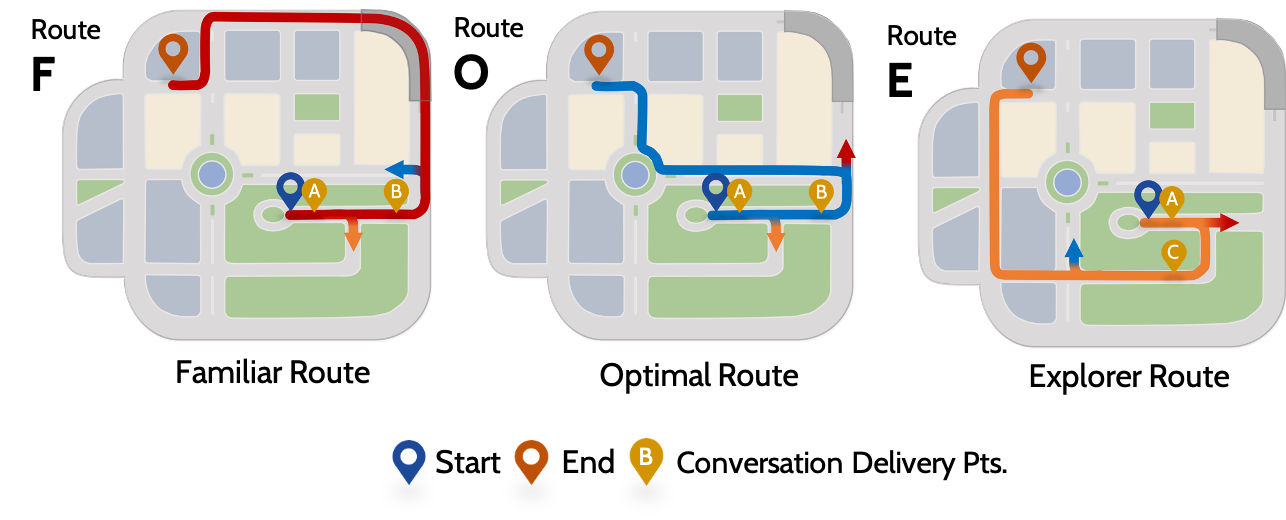
\includegraphics[scale=0.6]{figures/s2-all-routes.png}
  \caption{The selected routes from the map. The start and end points are the same for all routes. The orange markers are where the conversations are delivered, only once per trip. The 2 diverging arrows from each route show the alternative turns given in the conversations, colored to represent the type of route they lead to.}~\label{fig:s2-all-routes}
\end{figure*}

All routes in Figure \ref{fig:s2-all-routes} resemble a home-to-work trip and starts in the residential area of the map. They all had the same destination, which is opposite diagonally from the start point. This pair of points allowed us to identify the following routes based on Zhu \& Levinson and Tang \& Cheng's categories of trips that drivers usually take \cite{Tang2016AnalyzingData, Zhu2015DoPrinciple}.

\begin{itemize}
    \item \textbf{Route F} (Figure \ref{fig:s2-all-routes}b) - This route is straightforward and has a prominent landmark (i.e. a tunnel) that participants can easily remember and recognize \cite{antrobus_large_burnett_hare_2019}. 
    \item \textbf{Route O} (Figure \ref{fig:s2-all-routes}c) - This route uses the roundabout to avoid long waits at traffic signals \cite{Ringhand2017InvestigatingTime, Samson:2019:EFI:3290605.3300601}. It makes early turns compared to the Familiar route and is relatively the shortest among the three routes. 
    \item \textbf{Route E} (Figure \ref{fig:s2-all-routes}d) - This route is the longest and uses roads that are farther from the end pt on the other side of the map. This was based on the way modern apps suggest novel routes that are not short distance but algorithmically determined to be faster to avoid busy routes \cite{Samson:2019:EFI:3290605.3300601}.
\end{itemize}

\subsection{Voice Agents}
\label{sec:agents}

We created four voice agents that deliver turn-by-turn instructions to the participants, two for Route F and one each for Route O and E. 

\begin{table}[h]
	\centering
	\caption{The four voice agents, their assigned routes and their sample give turn-by-turn instructions.}
	\begin{tabular}{l l l}
	    \toprule
		\textbf{Voice} & \textbf{Route} & \textbf{Sample Instruction} \\
		\textbf{Agent} & & \\
		\midrule
		Generic & F & In 500 meters, turn left. \\
		Familiar & F & Let's turn left after 500 meters. We take that direction on most days. \\
		Optimal & O & We can turn left again in 300 meters. It will take us faster.  \\
		Explorer & E & Let's turn right. I think we haven't gone in this direction before. \\
		\bottomrule
	\end{tabular}
	\label{tab:agents}
\end{table}

Table \ref{tab:agents} shows the four voice agents used in this study, along with their assigned routes. All voice agents give out route descriptors for next turns and sometimes an absolute distance towards the next turn. The Generic voice agent give instructions patterned after the instructions commonly delivered by current navigation applications like Waze and Google Maps. Its phrasing is direct and authoritative (i.e. \textit{Turn Right} and \textit{Go Straight}). On the other hand, the Familiar, Optimal and Explorer voice agents are designed to sound more suggestive and promotes a partnership between the voice agent and the driver, mimicking the way a human collaborative navigator would give out instructions \cite{Antrobus2017Driver-PassengerSystems}. We also phrased them as such because we are aiming for a more suggestive tone so that drivers can have agency in making instructed actions, and for them to not panic as much when they miss turns \cite{Brown2012TheGPS, Samson:2019:EFI:3290605.3300601}. To achieve this effect, we designed them to always start their instructions with ``Let's,'' which is the shortest phrase we can add to the route descriptors without making them too long. 

Aside from the typical route descriptors, the instructions given by the Familiar, Optimal and Explorer voice agents also include the rationale for their suggestion. The Familiar voice agent says a phrase or sentence that reminds how regular the driver takes a road (i.e. We take that direction on most days). The Optimal voice agent adds a phrase or sentence to emphasize fastness or having less waits on traffic signals (i.e. It will take us faster). Lastly, the Explorer voice agent adds a phrase or sentence that highlights the novelty of the suggestion (i.e. \textit{I think we haven't gone in this direction before}). 

We first created the instructions in English. But because of the diversity of our participants who were recruited before the actual sessions, we eventually created versions in Filipino and Japanese languages, for a total of 12 voice agents. We translated the turn-by-turn instructions to Filipino and Japanese with the help of one Filipino and two Japanese native speakers.

We generated an audio file for each line of instruction using the Google Cloud Text-to-Speech API \footnote{https://cloud.google.com/text-to-speech/} because it supports our three languages with high-fidelity speech synthesis. Specifically, we used their WaveNet voice types. Since the voice agents will also be used in two-party conversations, we chose different voices and genders to differentiate them from each other. While previous works have shown that people have certain bias based on the gender of the voice agent \cite{Jeayeol2015}, we were limited to the voices available in the API. The English versions used two male (Familiar and Explorer) and one female (Optimal) voices. The Japanese agents also used two male (Familiar and Optimal) and one female (Explorer) voices. As a limitation of a low-resource language, the Filipino agents all used female voices which only varied by pitch -- high (Familiar, pitch=3.6), regular (Explorer, pitch=0) and low (Optimal, pitch=-3.2). The assignment of gender to voice agents was arbitrary. 

\subsection{Conversation Design}

\begin{table}[h]
    \caption{The conversation flow between the Familiar and Explorer voice agents when activated in the FE condition.}
	\label{tab:sample-convo}
	\centering
	\begin{tabular}{l l l}
	    \hline\hline
		\textbf{Turn} & \textbf{Voice} & \textbf{Instruction} \\
		\hline
		T1 & Familiar & ``Let's go straight and then turn left.'' \\
		T1 & Explorer & ``How about turning right before that?'' \\
		\hline
		T2 & Familiar & ``That's possible.\\ 
		& & But we take a left on most days.'' \\
		T2 & Explorer & ``That's true. But we haven't gone \\
		& & in this direction before.'' \\
		\hline
	\end{tabular}
\end{table}

The main goal of this study is to explore how turn-by-turn instructions delivered in two-party conversations affect the navigation choices of drivers. Following the Participation Framework \cite{Goffman1979-GOFF}, we assume the scenario of a driver driving with two collaborative passengers acting as navigators. Similar to Karatas et al. \cite{Karatas2018}, the driver participates as a bystander or a passive addressee to remove the conversational burden and to not distract the driver from driving. The active interlocutors are two voice agents which give different types of suggestions. 

We designed the conversations to have each voice agent speak in two turns, for a total of four turns. Each voice agent speaks in polite and friendly tones \cite{Yoshiike:2011:MSI:2177868.2177871} and acknowledges the suggestion of the other agent. The intention was to not make the conversation sound confrontational even though the voice agents may be presenting totally different suggestions. The voice agents split the typical route information they provide in two turns. They say their suggested direction in their first turn followed by their rationale in the second turn, and they do this alternately. 

Table \ref{tab:sample-convo} shows a sample conversation between the Familiar and Explorer voice agents in the FE condition. The first voice agent (Familiar) suggests a direction followed by a counter-suggestion from the second voice agent (Explorer). In most cases, the counter-suggestion is also phrased as a question (i.e. Explorer: ``How about turning right before that?''). In their second turn (T2), each voice agent shares the rationale behind their suggestion. They usually start with an affirmation or another question (i.e. Optimal: ``Are you sure? Turning left will take us faster''), followed by the rationale. All route information shared in conversations are the same as when they are giving suggestions by themselves (i.e. pure conditions).  

\begin{figure}[h]
\centering
  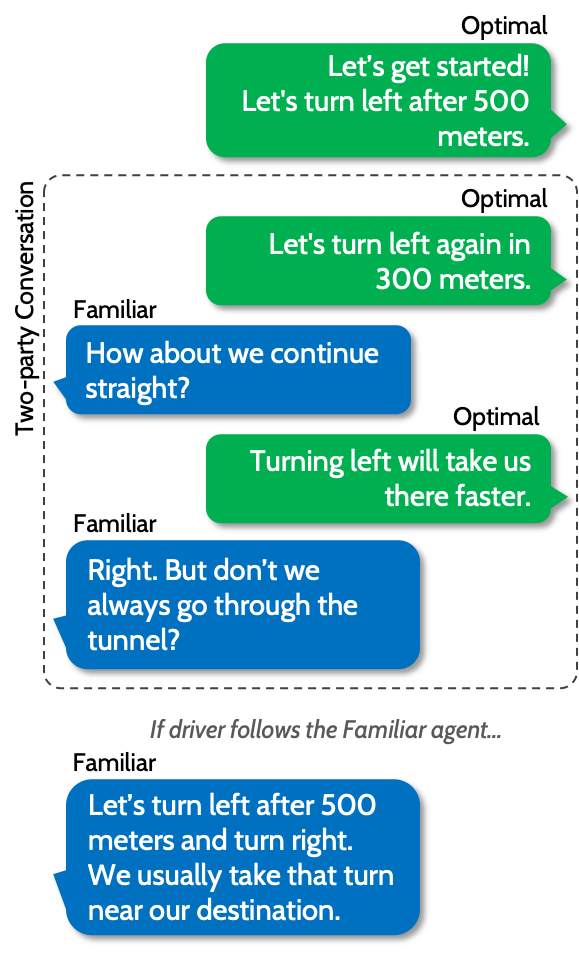
\includegraphics[scale=0.5]{figures/s2-convo.png}
  \caption{A sample sequence of turn suggestions given in the OF (\textit{Optimal-Familiar}) condition. It has a two-party conversation between the Optimal and Familiar voice agents. In this sequence, turn suggestions are first given by the 1st voice agent in the pair. They also start the conversation with the 2nd voice agent. After choosing a suggestion between the two, the trip continues with turn suggestions from the chosen voice agent, in this the Familiar.}~\label{fig:s2-convo}
\end{figure}

\subsection{Delivery as Voice Guidance}
In the conversation conditions, participants heard a conversation only once, which was either at the beginning or in the middle of the trip. Before a conversation, they heard only one voice agent giving route information. This is the first voice agent in the upcoming conversation. After the conversation is played, they continued hearing route information from the voice agent that they chose. Figure \ref{fig:s2-convo} shows the sequence of voice guidance for the whole trip in the OF condition. The voice guidance is started by the Optimal voice agent followed by the conversation. Assuming that the participant chose the Familiar suggestion, the voice guidance continued with the Familiar voice agent. Once they reach the destination, they heard the message ``We've arrived at our destination.'' If they deviate from the designed routes, there are also generic route information prepared for each voice agent (i.e. ``Let's turn left,'' ``Let's go straight.'').

\section{Method}

\subsection{Participants}
We recruited participants with at least 1 year of driving experience and has a driver's license mainly through word-of-mouth from a public university and local communities. Because not many students has a driver's license, we also used snowball sampling wherein our early participants recommended other people they know that fits our recruitment criteria. 

We successfully recruited 30 participants with an almost equal mix of people who identify as men (N = 16) and women (N = 14). Their ages range from 19 to 64 years old with an average of 29 (SD = 10.6). They comprise of 12 Filipinos and 18 Japanese nationals. The Filipino participants do not drive in their current place of residence but they drive in their country of origin. Thirteen of them are students while eleven are foreign workers. All participants do not drive as part of their occupation. When asked about their driving experiences, three have been driving for more than 10 years while the rest are only driving for 1 to 5 years. In terms of application usage, they have experienced using Google Maps (N = 25), in-car navigation systems (N = 8), Waze (N = 4) and NaviTime (N = 1). However, three of them have not used a navigation application before. Two Japan residents have been using these applications for more than 5 years while the rest are using them for less than 5 years. All of them use navigation applications only when going to an unknown destination and only one participant use it almost anywhere they go. When it comes to using voice guidance, 18 of them do not use it. For those that do, they frequently use it when they go on trips to new or seldom visited places.

\subsection{Setup}
The physical driving setup (Figure \ref{fig:s2-oz-setup}) uses one wide screen monitor and a Logitech G29 Driving Force steering wheel and pedals. On the other side of the table, the researcher sees a mirror of the participant's monitor. Every time the driver comes near a decision point, the researcher plays the recorded instructions and conversations. We used ordinary speakers for playing the voice guidance and this was placed in front of driver, positioned on their left. To record what the participants are saying while driving and thinking aloud, we also set up a GoPro Hero 7 that faces the driver. We only start recording once the actual driving sessions have started.

\begin{figure}
\centering
  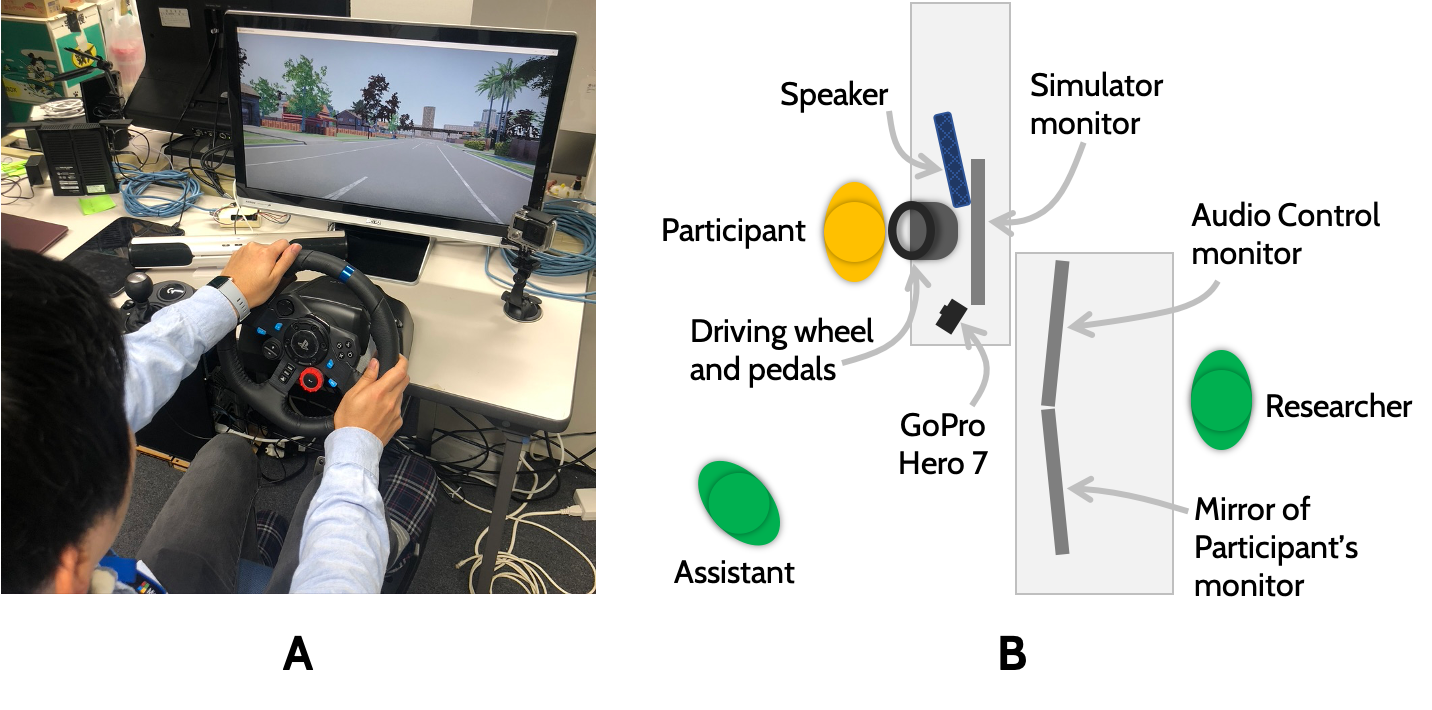
\includegraphics[scale=0.5]{figures/s2-oz-setup.png}
  \caption{The Wizard-of-Oz setup. [A] A participant driving in the virtual environment and [B] the overhead view of the room with the location of participant, researcher and assistant.}~\label{fig:s2-oz-setup}
\end{figure}

We used the open-source CARLA simulator \cite{Dosovitskiy17} as our virtual driving environment. We selected its Town3 map (Figure \ref{fig:s2-carla-map}) because of its grid-like layout with many options for alternative routes. The map also features distinct land use areas and buildings that participants can easily distinguish (i.e. residential, commercial and industrial areas) for easy orientation in the environment. The virtual driving environment was used as is. For every participant session, we generate 60 random vehicles of different types around the map and they drive autonomously. 

\begin{figure}
\centering
  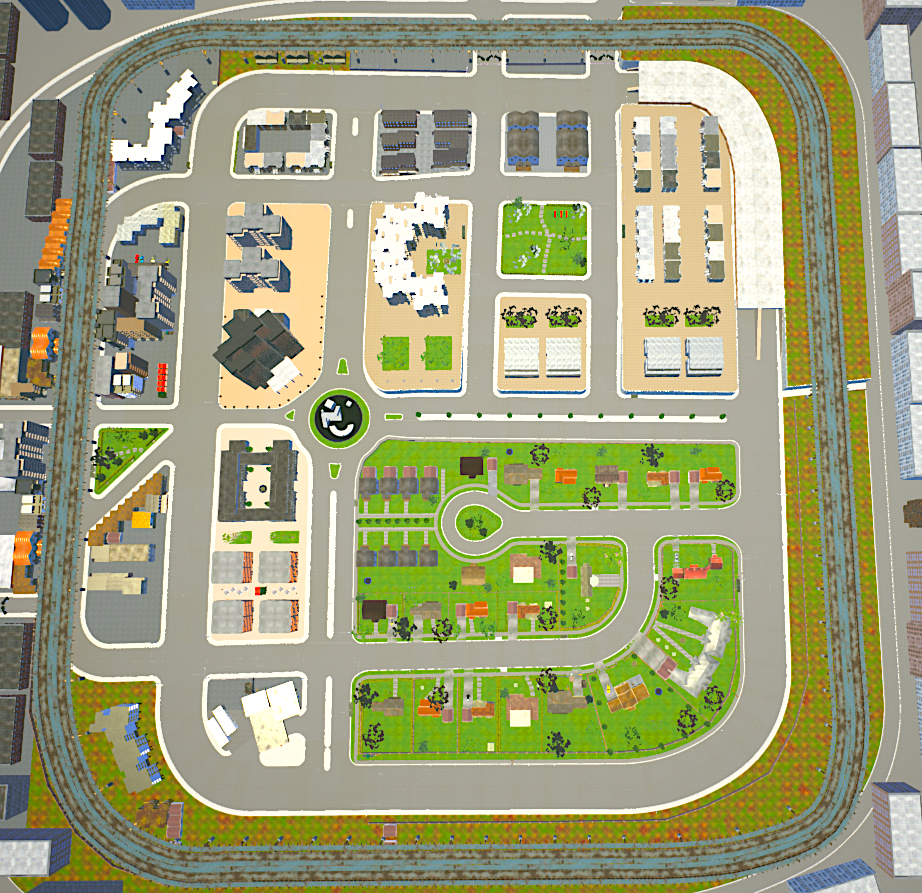
\includegraphics[scale=0.3]{figures/s2-carla-map.PNG}
  \caption{The Towm3 map of the CARLA simulator.}~\label{fig:s2-carla-map}
\end{figure}

\subsection{Conditions}
Using the routes discussed in the \nameref{sec:routes} subsection, we designed the study to have three pure conditions and 6 conversation conditions. The pure conditions use only one voice agent namely and does not play any conversarions, \textit{PF} for Familiar voice agent only, \textit{PO} for Optimal voice agent only, and \textit{PE} for Explorer voice agent only. The conversation conditions use combinations of voice agents and are named the following: \textit{FO} (Familiar+Optimal), \textit{FE} (Familiar+Explorer), \textit{OF} (Optimal+Familiar), \textit{OE} (Optimal+Explorer), \textit{EF} (Explorer+Familiar) and \textit{EO} (Explorer+Optimal). The suggestion of the 2nd agent in conversations is the expected choice (\textit{appropriate}).

\subsection{Protocol}
We conducted a within-subject Wizard of Oz study which tasks each participant to drive 9 times under different navigation conditions. To reduce any ordering effect, we prepared 30 randomly ordered sequences of the 9 conditions and randomly assigned the participants to them. 
In the room, there is the participant and the experimenter. For the Japanese participants, a Japanese student assistant who is knowledgeable about the study and can translate English to Japanese is also present. For the duration of the actual driving sessions, the experimenter and assistants cannot talk nor react to the participant. 

\subsubsection{Orientation} 
At the beginning of each session, we briefed them about the project and the purpose of the experiment they are about to perform. Then, we obtained their consent to the procedures of the study and their answers to a pre-trial questionnaire that asks about their demographic information, driving background and experience with using navigation applications and voice guidance. Then, we oriented them about the steering wheel and pedals, and the simulation environment. For Japanese participants, it was emphasized that the environment is configured for driving on the right side of the road, which was different from what they are used to. We also mentioned the presence of a roundabout which does not exist in Japanese roads. During the whole orientation, we showed them a map. We gave them 3 minutes to drive around and get comfortable with the controls. 

\subsubsection{Familiarization with Voice Agents} 
After they became comfortable with the controls and environment, we asked what language they prefer for the voice guidance. All participants chose to use the local language versions, with nobody using the English voice guidance. We told them that they will hear 3 types of voices during the driving sessions and then played them the synthesized voices. Each voice was assigned a name and a number just for this step. To check how well they can differentiate the voices, we played them again but this time, they had to tell which voice was speaking (i.e. first voice, Tanaka-san, Olive). This step was done in order for them to easily detect when a conversation is being played already.

\subsubsection{Remembering a Regular Route}
Once they are familiar with the voices, the next step required them to familiarize with a route that served as their regular route to the destination. We showed them a map with the route drawn in red and they made two trips in the simulation following it. We played voice guidance so they can focus on the road and practice hearing the guidance. After this, they were asked to drive again to the destination but without voice guidance. In this step, we wanted to check how familiar they were with the route we asked them to follow. Once they reach the destination, we asked them to rate how good they think the route is, 1 being very bad and 7 for very good. For this question, we wanted to know later if their score affects how often they follow this route.

\subsubsection{Trial of NASA-TLX} 
Since this was the first time that the participants have done this kind of study, we gave them a trial. We asked them to rate their workload using the NASA Task Load Index (TLX) questionnaire after following the voice guidance in the route familiarization step. 

\subsubsection{Driving Sessions} 
Each participant drove 9 times. Before anything, we reminded them that they are not obliged to follow the directions given by the voice guidance. After hearing the suggestions and conversations, it is up to them to decide which direction to go based on the given scenario and their personal preference. At the beginning of each drive, they were told to forget their previous drives and assume that they are hearing the voice guidance for the first time. They were also asked to think aloud. While we were starting their environments, we told them to internalize one of the following scenarios: 

\begin{table}[h]
	\centering
	\caption{The different scenarios given to the participants before each condition.}
	\begin{tabular}{l l}
		\toprule
		\textbf{Scenario} & \textbf{Description} \\
		\midrule
		Regular Day & It is a regular day. You woke up on time \\
		& and you have your regular schedule at the \\
		& destination. \\
		In a hurry & You have a meeting in the morning and \\
		& you overslept. You are already running late. \\
		Lots of time & You have no morning meetings but you \\
		& woke up very early. You now have more\\
		& time to spare. \\
		\bottomrule
	\end{tabular}
	\label{tab:scenario}
\end{table}

Each scenario in Table \ref{tab:scenario} corresponds to a set of conditions. The Regular Day scenario is given in the PF, OF and EF conditions while the In a hurry scenario is given in the PO, FO and EO conditions. Lastly, the Lots of time scenario is given in the PE, FE and OE conditions. After each drive, they answered a post-task questionnaire that includes questions discussed in the \nameref{sec:post-task} subsection. They can choose to have a break anytime during each session. After all 9 drives, they accomplished the Source-of-Workload Comparison sheet to complete the workload assessment. Each session lasted around 75 to 90 minutes.

\subsection{Post-Task Questionnaire}
\label{sec:post-task}
First, participants assessed their amount of workload using the standard NASA TLX questionnaire. We did not use a modified version like in Karatas et al. \cite{Karatas2018} because this study does not intend to measure driving workload per se. To focus their assessment, we asked participants to assess based on the following aspects of the navigation task: a) listening to the voice guidance, b) choosing a direction after hearing the agents, and c) checking where to make the turn. The questionnaire was translated to Japanese following the work of Miyake \cite{MIYAKE2015}. Additionally, participants shared the reason behind their navigation choices (free text field) and how confident they were after choosing them (from 1 to 7).

\section{Results}

\subsection{Unanticipated Challenges}
We begin by discussing some challenges we encountered in running this study. While the driving in the simulation environment, there were multiple instances that we had to restart because the vehicle will not move. Usually at the beginning after they have heard the first voice guidance, they would notify us. This happened at most 5 times for one participant and five participants experienced this at least once. 

We chose the simulation tool because we wanted to control the number of other vehicles, putting the participants in a more realistic driving environment. However, because the other vehicles are stochastic, there was one instance wherein we had to restart the environment midway because of a traffic jam. In that moment, our prepared audio files for voice guidance were not enough to direct the participant out of the traffic jam. But instead of immediately running that same condition, we changed the order so that the participant can forget the given instructions.

\subsection{Impact on Choices}
In this study, one of our main goals is to explore the impact and limitations of adding conversations in making navigation choices. We analyzed how associated their choices were for each given scenario and condition, along with a discussion of their reasons, and then discuss how combinations of these voice guidance affected their choices. 

\begin{figure}
\centering
  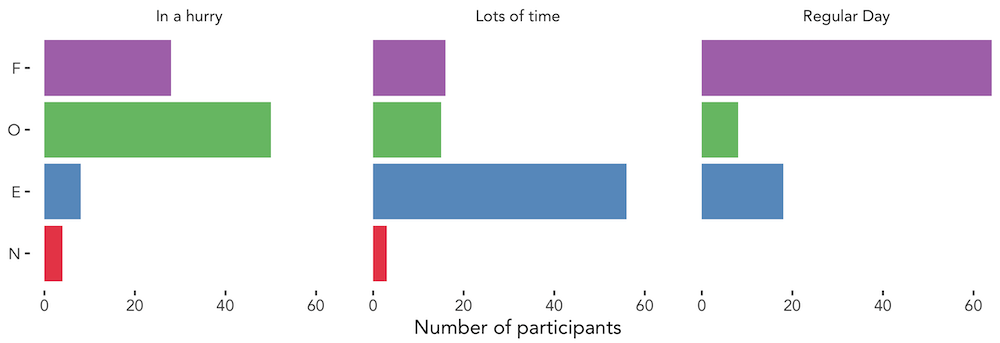
\includegraphics[scale=0.4]{figures/s2-choice_per_scenario.png}
  \caption{Distribution of navigation choices per scenario. D refers to those who chose the Familiar suggestion, O for Optimal suggestion, E for Explorer suggestion, and N for those who chose neither of the given suggestions.}~\label{fig:scenario-choice}
\end{figure}

First, we wanted to see how aligned the participants' choices were based on the scenario that was given to them at the beginning of each condition. We tallied the participants' choices and found that all types of suggestion were chosen at least once by the participants in each scenario (Figure \ref{fig:scenario-choice}). Looking at the contingency table of choices versus scenario, a chi-square test shows that choices made by participants are dependent on the current context of their driving ($\chi^2$ = 123.35, p < 0.05). 

Examining this association further, a chi-square test of the breakdown of choices made by participants under each condition (Figure \ref{fig:cond-choice}) shows that the type and combination of voice guidance was associated with their navigation choices ($\chi^2$ = 229.87, p < 0.05). Many participants navigating under the PF, FO and OF conditions were likely to choose the Familiar suggestion, while those under the PO and EO conditions were likely to choose the Optimal suggestion. In the PE, EF and FE conditions, participants were attracted to choosing the Explorer suggestion, while both Optimal and Explorer suggestions were positively associated with the OE condition.

\begin{figure}
\centering
  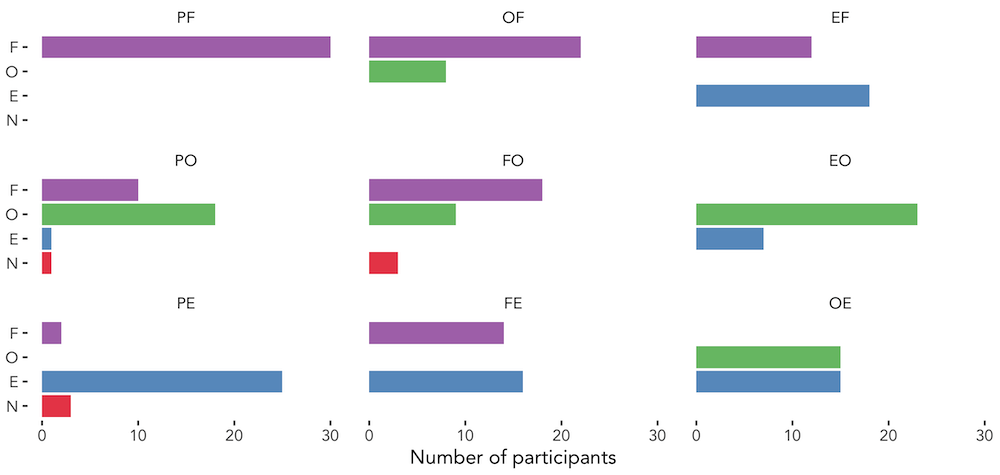
\includegraphics[scale=0.4]{figures/s2-choice_per_condition.png}
  \caption{Distribution of navigation choices per condition. The first row shows the conditions under the \textit{Regular Day} scenario, followed by the conditions in the \textit{In a hurry} and \textit{Lots of time} scenarios.}~\label{fig:cond-choice}
\end{figure}

\subsubsection{Regular Day Conditions}
Given the prompt in the Regular Day scenario, the Familiar suggestion comprise almost 3/4 of the choices (N = 64) suggesting a strong association. And although there were those who chose the Optimal scenario, it was only chosen 8 times across the three conditions (PF, OF, EF). 

In the PF condition, all 30 participants chose the Familiar suggestion. Four participants chose it primarily because the voice agent always reminded them of how often they take the suggested roads (P17, P20, P21, P30) while three participants add that it is because that is the only given suggestion (P11, P20, P28). Two participants also cited trust because ``\textit{it knows the way, [there is] no need to think}'' - P19. Participants also felt at ease (P9) that they can arrive at the destination without thinking (P5, P7, P28) because of the easy-to-understand road navigation (P18, P27). Six participants also felt it appropriate because they ``\textit{...have nothing to do or [they are] not in a rush}'' (P15). Interestingly, one participant chose it because they ``\textit{don't want to go the other way because I might get lost}'' - P23.

When suggestions were given in two-party conversations (OF and EF), their positive association with the Familiar suggestion was only maintained in the OF condition. Even in a two-party conversation with the Optimal voice agent, participants still chose the Familiar suggestion because they thought it was correct (P12), easier to follow (P7, P22-23) and familiar (P13, P16, P18, P26). They also chose it because they were not in a rush to go to their destination (P14-15). Commenting against conversations, two participants chose the Familiar route because they found the conversations confusing (P6, P9) leading them to default to a suggestion they felt at ease with. On the other hand, two participants shared that they would have followed the Optimal suggestion had its rationale been delivered earlier in the conversation (P19, P29). For those that did choose the Optimal suggestion, P20 thought that it was easier to follow compared to the Familiar suggestion — without much elaboration, while three other participants were mostly in agreement with the rationale spoken by the Optimal voice agent (P4, P11, P27). Two participants found it an opportunity to explore a new route because they were not in a rush (P10, P17) while another two participants chose the Optimal suggestion because it was the first thing they heard from the conversation. 

In the EF condition, more participants chose the Explorer suggestion (N = 18) than the Familiar suggestion. They did not see it as a bad choice (P30) while some actually chose it because they wanted to explore a new route (P4, P6-7, P20, P24-25, P27) and they had ample time (P18, P26). Like in the OF condition, there were also participants that chose the Explorer suggestion because it was the first one they heard (P5, P8, P15, P19). Familiarity is still the main reason of the six participants that chose the Familiar suggestion, while three others chose it because they think they have plenty of time. Interestingly, P13 and P22 chose the Familiar suggestion, and P12 and P28 chose the Explorer suggestion because they all thought their choices were faster. This was their criteria despite having no time constraint in the Regular Day scenario. 

\subsubsection{In a hurry Conditions}
In the In a hurry scenario, participants were most attracted to choosing the Optimal suggestion with more than half of the choices made (N = 50). However, almost a third (N = 28) of the choices were still Familiar suggestions, indicating participants' tendency to default to regular routes even though they were in a hurry \cite{Samson:2019:EFI:3290605.3300601, Zhu2015DoPrinciple, Tang2016AnalyzingData}. 

In the PO condition, more than half of the participants chose the Optimal suggestion (N = 18) primarily because they believed that the suggestion will take them faster towards the destination. P12 adds that they followed the suggestion because there is ``\textit{no hassle, [and it is] no[t] much effort.}'' Highlighting the benefit of hearing why they were given that suggestion, P27 shares that ``\textit{The usual way was good, but I did not have time. I got it when it taught the shortest way, so I went to the shortest way as instructed.}'' On the other hand, two participants shared that they were unsure where to go especially when the instruction ``\textit{Let's turn left again in 300 meters}'' was given to them. This suggestion is played immediately after they make the first left turn at decision point B. P10 was not sure when to make the next turn: ``\textit{I didn't know where [is] 300 meters away.}'' Additionally, P5 was ``\textit{suddenly confused when told to go left. I ignored it because it was a little over.}'' Hence, while the rationale behind the suggestion was appreciated and encouraged participants to follow, the addition of the distance information made it confusing for others \cite{Antrobus2017Driver-PassengerSystems}. This resulted to them following the Familiar suggestion instead. Aside from being comfortable with the Familiar route (P23), two other participants chose the Familiar suggestion because they thought it was faster than the Optimal suggestion \cite{Peterson2018}.

After listening to a two-party conversation in the FO condition, the number of participants who chose the Optimal suggestion drops to less than a third in the pure condition (N = 9). Participants had the same reasons why they continued to follow the Optimal suggestion (i.e. belief that it is faster, with less waits). On the other hand, two participants chose the Familiar suggestion because they got confused while listening to the conversation: ``\textit{Two agents were proposing many ways along the way, and I couldn't understand what they were saying, so I went to the usual road while listening to the suggestions}'' - P27. Speaking about the timing and length of conversation, four participants eventually followed the Familiar suggestion because it was already too late for them to make the turn suggested by the Optimal voice agent. ``\textit{After listening to the conversation between the agents, I couldn't turn to get there quickly}'' - P29. Lastly, the rest of the participants did not believe the Optimal voice agent's rationale and thought the the Familiar suggestion is still faster.

Having the opposite effect, participants in the EO condition followed the Optimal suggestion the most number of times in the In a hurry scenario (N = 23). This time, most of the participants agreed with the rationale of the Optimal voice agent and decided that it was more appropriate. However, when we traced their complete trips after following the Optimal suggestion from the conversation, five participants eventually followed the familiarization route, not the optimal route. This suggests that even though they agreed with the suggestion and thought it will take them faster, familiarity was still a contributing factor. 

\subsubsection{Lots of time Conditions}
In the Lots of time scenario, they mostly chose the Explorer suggestion (N = 56) when they were told that they had much time to spare. This preference was consistently observed in the PE condition wherein 25 of them chose the Explorer suggestion. Two participants (P6, P8) followed it because that was the only suggestion given while six others were just open to the suggestion given the scenario they are in (P10, P12, P18, P24, P26, P29). There were also some participants who really wanted to explore new routes that they can use in the future: ``\textit{I chose to go that route so that I can expand my knowledge of the different ways I can get to work}'' - P16. For those who chose otherwise, one participant ignore the Explorer suggestion and drove the familiar route because ``\textit{the agent says turn right twice instead of left to pass the tunnel. Wrong direction}'' - P25. Interestingly, three other participants completely went their own ways.

When the Explorer suggestion was given in the FE condition, there were less participants who chose it because they were also reminded with the Familiar suggestion. Focusing on participants who chose the Familiar suggestion, they cited reasons of familiarity (P7, P14, P20-21, P28) and correctness (P12). Interestingly, two participants who chose the Explorer suggestion in the PE condition now followed the Familiar suggestion because ``\textit{I'm not confident about the other road}'' - P4. 

In the OE condition, participants were evenly split between the Optimal and Explorer suggestions. Everyone who chose the Explorer suggestion are driven by the non-urgency of the scenario, making them more open to explore new routes. However for those who chose the Optimal suggestion, while they also considered the non-urgency of the situation, they prioritized comfort (P12, P20, P23) and familiarity (P14, P21, P23, P28) in choosing. In addition, P30 did not choose the Explorer suggestion because ``\textit{it is not good to go on a road that [the] Navi does not know}.'' This impression might have been because the Explorer voice agent says this as one of its suggestions: ``\textit{Let's turn right. I think we haven't gone in this direction before.}''

\subsubsection{Goodness of Familiarization Route}
At the beginning of each study session, we asked the participants to rate how good the familiarization route is. Out of the 27 participants who were able to do so, 23 of them gave good ratings (between 5-7) while only four gave low scores of 3 and 4.  

We found that participants who rated it as good were following it more than we expected. In the PO and PE conditions, eight and two participants followed the Familiar suggestion respectively even though there was no mention of Familiar suggestion in the voice guidance. However, looking at the association between choice and their goodness rating, a chi-square test shows that they are actually independent of each other.

\subsection{Impact on their Confidence with Choices}
Overall, confidence in their choices was generally lower when suggestions were given in conversations. When the \textit{Familiar} suggestion was given on its own (PF condition), average confidence was 5.9 (M = 6.5, $\sigma$ = 1.41) -- the highest among conditions -- with half of the participants giving a score of 7. Compared with other conditions given in the \textit{Regular Day} scenario, their average confidence then drops to 5.6 for the OF condition (M = 6, $\sigma$ = 1.7) and 5.4 for the EF condition (M = 5.5, $\sigma$ = 1.5).

\begin{figure}
\centering
  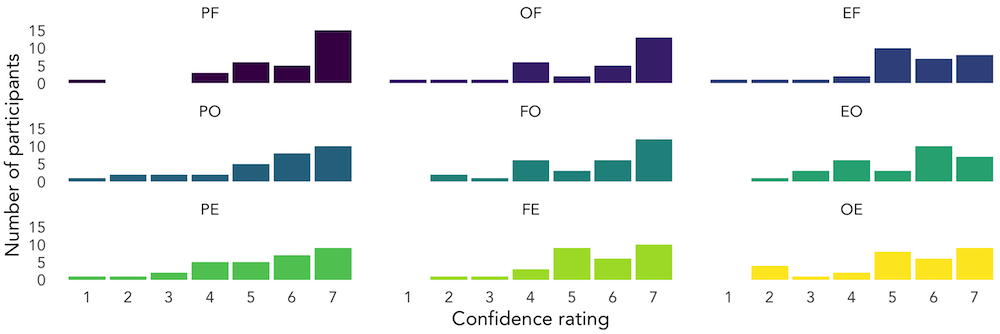
\includegraphics[scale=0.4]{figures/s2-confidence_per_condition.png}
  \caption{Distribution of confidence rating per condition. The first row shows the conditions under the \textit{Regular Day} scenario, followed by the conditions in the \textit{In a hurry} and \textit{Lots of time} scenarios.}~\label{fig:cond-conf}
\end{figure}

When participants heard suggestions that are different from what they are familiar with, they self-reported relatively lower confidence with their choices. Under the \textit{In a hurry} scenario, their average self-reported confidence was 5.4 (M = 6, $\sigma$ = 1.73) when they only heard the \textit{Optimal} suggestion (PO condition). This was slightly lowered to 5.3 (M = 6, $\sigma$ = 1.47) when they heard it with the \textit{Explorer} suggestion. In the \textit{Lots of time} scenario, they had average confidence ratings of 5.3 (M = 6, $\sigma$ = 1.64) and 5.27 (M = 5.5, $\sigma$ = 1.68) when they only heard \textit{Explorer} suggestions and when it was mixed in a conversation with the \textit{Optimal} suggestion. 

The only increases happened when the familiar route suggestion was also given in conversations in the FO ($\mu$ =  5.5, M = 6, $\sigma$ = 1.6) and FE ($\mu$ =  5.6, M = 6, $\sigma$ = 1.3) conditions compared to when it was only the \textit{Optimal} and \textit{Explorer} suggestions mentioned. These suggests that the addition of novel suggestions, \textit{Optimal} and \textit{Explorer}, in conversations for all scenarios negatively affects how they perceive their choices. However we are not yet certain whether they actually felt less confident after making a wrong choice or even with the right choice for the scenario. Additionally for all scores, there are no significant differences after a Wilcoxon Signed-rank test.  

\subsubsection{High Confidence on Familiar and Optimal Suggestions}
Based on a chi-square test, the self-reported confidence of drivers are choice-dependent ($\chi^2$ = 23.90, p < 0.05). In trips where the \textit{Familiar} suggestion was followed (N=108), participants had an average confidence rating of 5.58 and this choice has a positive association with the confidence rating of 7, primarily because it is what they are already familiar with.

For all \textit{Regular Day} scenario trips, participants who chose the \textit{Familiar} suggestion were more confident (N=64, $\mu$ =  5.84, M = 6). In the OF condition, while many trips chose the \textit{Familiar} suggestion (N = 22) over the \textit{Optimal} suggestion (N = 8), participants were equally as confident in choosing the \textit{Optimal} suggestion ($\mu$ =  5.6, M = 6.5, $\sigma$ = 1.85) compared to choosing \textit{Familiar} ($\mu$ =  5.5, M = 6, $\sigma$ = 1.68). Due to the low stakes nature of the scenario, even though the participants chose an unnecessarily faster suggestion, they did not mind it as much unlike when they chose the totally novel \textit{Explorer} suggestion ($\mu$ =  4.89, M = 5) overall. The low stakes nature of the \textit{Lots of time} scenario also made participants more confident in following \textit{Familiar} even though it was followed less often (N=16, $\mu$ =  5.63, M = 6) and intentionally less appropriate compared to the \textit{Explorer} suggestion (N=56, $\mu$ =  5.23, M = 5). However in the \textit{In a hurry} scenario, confidence with the \textit{Familiar} suggestion was remarkably lower ($\mu$ =  4.96, M = 5) even though it was chosen by participants in 47\% of the trips in the PO and FO conditions.

Despite being chosen the least among the three suggestions, the \textit{Optimal} suggestion (N=73) was still positively associated with high confidence ratings of 6 to 7. This is can be attributed to the fact that the \textit{Optimal} and \textit{Familiar} suggestions are identical (\textit{``Turn left after 500 meters''}) except for the rationale said. Overall, participants reported an average confidence of 5.75 after choosing the \textit{Optimal} suggestion.

In the \textit{In a hurry} scenario, participants who chose the appropriate \textit{Optimal} suggestion reported a 5.8 average confidence (N=50, M = 6) which was consistently the highest in the PO ($\mu$ =  5.94, M = 6, $\sigma$ = 1.3), FO ($\mu$ =  6.33, M = 1, $\sigma$ = 1) and EO ($\mu$ =  5.48, M = 6, $\sigma$ = 1.27) conditions. Half of the participants were also confident with choosing the \textit{Optimal} suggestion in the OE condition ($\mu$ =  6.33, M = 1, $\sigma$ = 1) despite it being the less appropriate choice. However, despite choosing the \textit{Optimal} suggestion, eight (8) of them never really followed the complete \textit{Optimal} route and went on to follow the familiar route instead. So this suggests that they were confident in their choice not because they thought choosing a faster route was correct but more because of their familiarity with the turn.

\subsubsection{Low Confidence for Explorer Suggestion}
Choosing the \textit{Explorer} suggestion is strongly positively associated with the confidence rating of 5 and strongly negatively associated with confidence rating 7. The novel nature of the suggestion made drivers less confident in their choices. This is consistent with previous works. Participants also felt unsure whether they will receive continuous guidance if they deviate from the familiar route.

After choosing the \textit{Explorer} suggestion in the \textit{Lots of time} scenario, participants reported average confidence scores of 5.12 in the PE condition (M = 5, $\sigma$ = 1.67) and 4.87 in the OE condition (M = 5, $\sigma$ = 1.41). Their confidence was low despite choosing the \textit{Explorer} suggestion 67\% of the time for both conditions. Only in the FE condition did the participants felt more confident with following the \textit{Explorer} suggestion ($\mu$ =  5.75, M = 5.5, $\sigma$ = 1), but still not as much compared to the \textit{Familiar} and \textit{Optimal} suggestions.

\subsubsection{Choosing Alternatives}
 We also looked at how confident the participants were when they chose the alternative suggestion over the appropriate ones. In the EF condition, participants started self-reporting low confidence scores of 1 to 4 (N = 4) after choosing the \textit{Explorer} suggestion ($\mu$ =  4.89, M = 5, $\sigma$ = 1.57) compared to those that chose the \textit{Familiar} suggestion, who mostly reported scores between 5 to 7. In the \textit{Regular Day} scenario, we expect them to prefer the \textit{Familiar} suggestion over the \textit{Explorer} one. It shows that even though they made a wrong choice, they must have realized after performing the task that they should have chosen the \textit{Familiar} suggestion instead. The same lower level of confidence was also reported after participants chose the \textit{Familiar} suggestion in the FE ($\mu$ =  5.43, M = 6, $\sigma$ = 1.65) and FO ($\mu$ =  5.11, M = 5, $\sigma$ = 1.75) conditions. They were not expected to prefer the \textit{Familiar} suggestion, but 14 and 18 participants did in the FE and FO conditions respectively. And although some of them self-reported scores of 6 to 7 --- because they are familiar with it --- we also observed more participants reporting lower scores from 2 to 4 ($N_{FE}$= 4, $N_{FO}$= 7). 

\subsubsection{Good and Bad Pairs}
Pairing novel suggestions in conversations made participants less confident with their choices even when they made appropriate ones. Participants in the EO condition who chose the \textit{Optimal} suggestion reported confidence scores ($\mu$ =  5.48, M = 6, $\sigma$ = 1.27) with seven of them giving scores between 3 and 4. This  is lower compared to when they chose the same suggestion in the PO condition ($\mu$ =  5.94, M = 6, $\sigma$ = 1.30) with only two participants reporting scores between 2 and 4. This was also the case in the OE condition where the average confidence score of 4.87 (M = 5, $\sigma$ = 1.41) after choosing the \textit{Explorer} suggestion was lower compared to the 5.12 average confidence score in the PE condition (M = 5, $\sigma$ = 1.67). Four more participants gave scores between 1 and 4 in the OE condition. This is consistent with previous works that highlighted people's tendency to not prefer suggestions when they are too novel, putting them under a lot of uncertainty \cite{Ekstrand2014UserAlgorithms}. 

On the other hand, the delivery of the \textit{Familiar} suggestion as an alternative in the FO and FE conditions made participants feel more confident in choosing the \textit{Optimal} and \textit{Explorer} suggestions. Even though less participants chose the \textit{Optimal} suggestion in FO (N=9) compared to PO (N=18), and the \textit{Explorer} suggestion in FE (N=16) compared to PE (N=25), they felt relatively more confident with average scores of 6.33 (M = 7, $\sigma$ = 1) and 5.75 (M = 5.5, $\sigma$ = 1) respectively. Including the \textit{Familiar} suggestion gave participants a recognizable point of comparison. This was in contrast to their experience in the all-novel conditions (EO, OE) wherein they had to process two new suggestions and also recall their regular choices.

\begin{figure}
\centering
  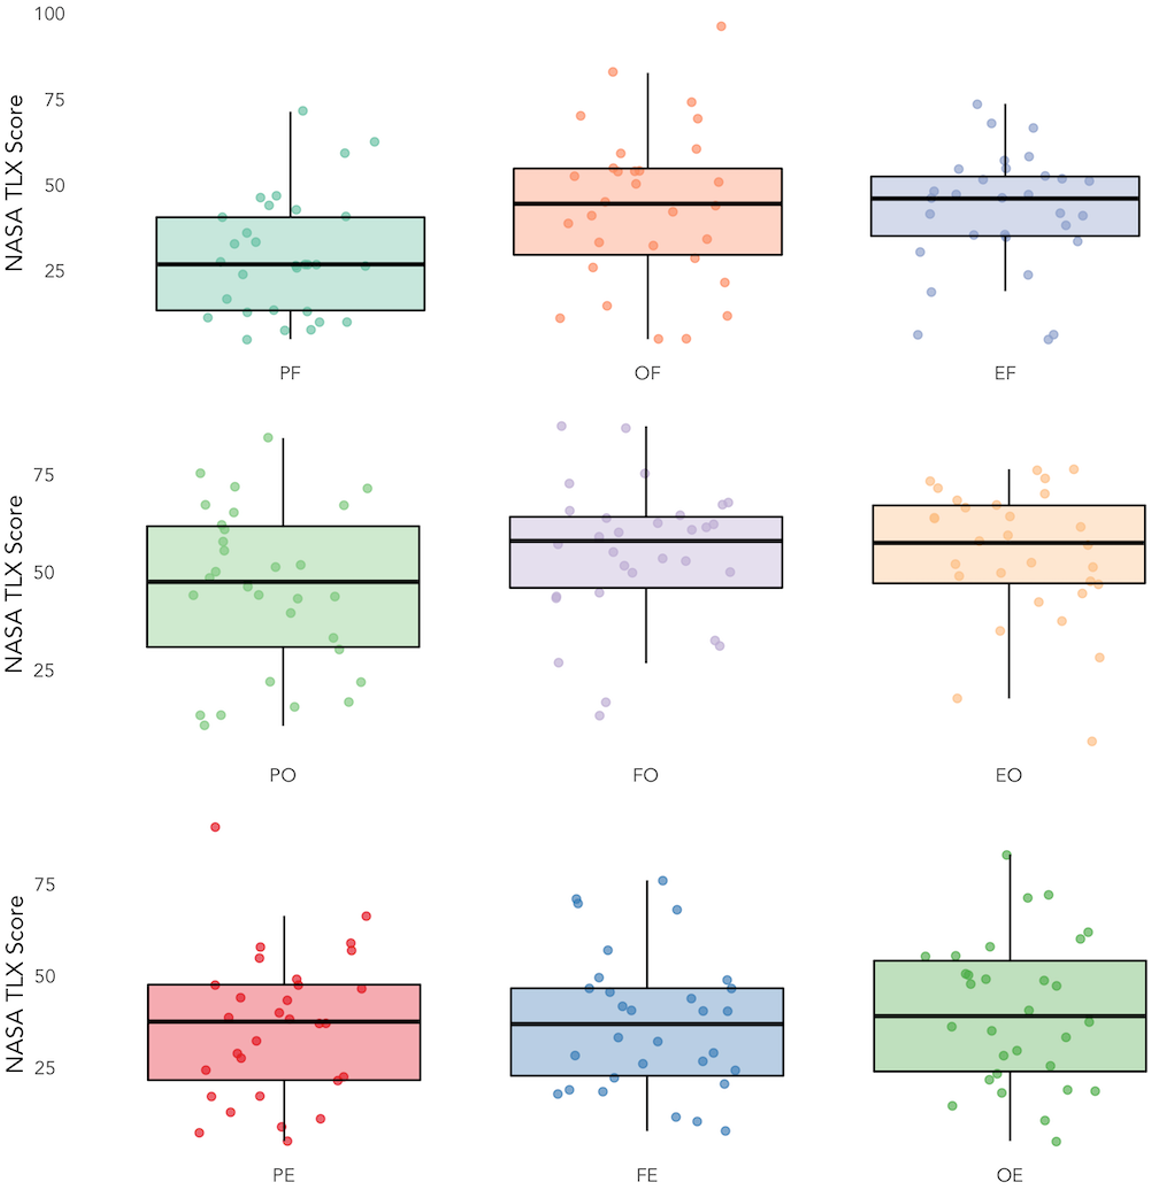
\includegraphics[scale=0.7]{figures/s2-workloads.png}
  \caption{NASA TLX scores of each participant after each condition. The first row shows the conditions under the \textit{Regular Day} scenario, followed by the conditions in the \textit{In a hurry} and \textit{Lots of time} scenarios.}~\label{fig:workloads}
\end{figure}

\subsection{Impact on Workload}
Because our concept gives more information than the typical voice guidance, we wanted to see how much the two-party conversations impact the workload of the participants. Figure \ref{fig:workloads} shows the NASA TLX scores of the 30 participants in each of the conditions. A box plot is superimposed on each dotplot. The total NASA TLX scores show that the PF condition (M = 26.84, $\sigma$ = 17.31) resulted to less workload compared to the PO (M = 47.5, $\sigma$ = 20.8) and PE (M = 37.5, $\sigma$ = 19.86) conditions. In Student's Paired lower-tailed t-tests between PF and PO, and PF and PE, p<0.001 and p<0.05 respectively, indicating significant decrease in the PF condition. Comparing between PO and PE, a Student's Paired upper-tailed t-test resulted in p<0.01 indicating a significant increase in workload for the PO condition.

Internalizing the Regular day scenario, participants reported higher workloads when the Familiar suggestion was mixed in conversations. Both EF (M = 46, $\sigma$ = 17.34) and OF (M = 44.5, $\sigma$ = 22.76) show significant increases in a Student's Paired upper-tailed t-test with p < 0.001. This increase must have been because they had to recall the first suggestion which was relatively new to them. Suggesting the regular route must have distracted them into considering the new suggestions. Although that does not seem to be the case in the EF condition wherein more participants chose the Explorer suggestion.

Compare to the PO condition in the In a hurry scenario, workload increased for both FO (M = 58, $\sigma$ = 17.73) and EO (M = 57.5, $\sigma$ = 17.1) conditions. However, after a Student's Paired t-test with the FO scores and a Wilcoxon Signed-rank test with the EO scores, only the FO condition showed a significant increase with p < 0.05. This was mainly due to the short amount of time between the moment the conversation was played and the point where they had to make a turn, which was a limitation of our concept design and chosen simulation environment.

When navigating under the Lots of time scenario, participants reported almost similar workloads for the Pure Explorer, FE (M = 36.83, $\sigma$ = 18.61) and OE (M = 39, $\sigma$ = 19.75) conditions, and a Student's Paired t-test did not show significant differences between them. Although the conversations did not significantly increase the workload, this somehow suggests that participants were consistently challenged considering the Explorer suggestion because of its novelty.

\section{Towards Better Voice Guidance}

This study provides initial insights into how voice guidance delivered as two-party conversations can impact the way drivers make navigation decisions. Here we present a summary of key findings from the results and provide design considerations for future iterations of navigation applications and recommender systems, in general.

\subsection{Supporting Instructed Actions}
Just by looking at the distribution of navigation choices made by participants, we can see clear patterns of choices being made in the pure conditions than in the conversations. When alternative suggestions get mentioned, their choices changed as well. While this can be considered as a negative result, we see it supporting our initial goal of encouraging drivers to have instructed actions \cite{Brown2012TheGPS}. Although we designed our scenarios to give more reasons for the participants to choose and follow certain suggestions (i.e. We expect the Optimal suggestion to be chosen more in the In a hurry scenario), we certainly do not consider choosing the alternative suggestions as a wrong decision. Our intent is to design and explore a new technique that will empower them with a handful of choices, rather than constrain them into following something that was already decided for them.

From the video recordings of their sessions, we observed them listening completely to the conversations, with some participants even slowing down a bit to focus on what was being said. When they shared their reasons why they made those choices, we observed more comparative and convinced answers, with some of them even citing the voice agents. The way the voice agents took turns and built up the conversation also made them feel convinced about the correctness of both suggestions. For example, P19 shared that they ``heard the second agent. I just felt more confident with the first agent because in the end, the second agent agreed with the first agent's suggestion.'' Participants were encouraged to believe that both suggestions are true and they have the ability chose whichever they prefer or feel is appropriate for the situation.
However, this approach also brings the challenge of drivers having too much affinity with the voice agents. Based on the shared reasons and utterances from the video recordings, some participants felt less confident with the Explorer voice agent because it says the phrase ``I think we haven't gone in this direction before.'' It made them think that it will not know where to go if they follow its suggestion. While the design intent was for the voice agent to remind the driver of what roads it has and has not taken before, the driver's affinity made it think they know the same things. 

\subsection{Order, Timing and Amount of Information}
One of the main challenges in this concept is time criticality. Recommender systems giving multiple options is not uncommon. Even for navigation applications and in-car navigation systems, they allow drivers to browse through alternative routes. However, they do so in situations and tasks that allow time for their users to choose. In our Wizard of Oz study, the slow reveal and the amount of information in the conversations made it less effective in certain decision points like in the FO and OF conditions. Future work might want to consider combining the direction information and the rationale in one turn. This will allow drivers to ascertain immediately whether they should follow the suggestion or not. Then, it can be delivered in two turns instead of four like in the current concept. For turns that will be made in close distances, we suggest removing distance information (i.e. ``in 300 meters'') and fixing the order of suggestions in the conversation. In the FO condition, the Optimal suggestion is said after the Familiar suggestion, and its rationale on the last turn. This made some drivers feel it is too late and they ignore the Optimal suggestion despite being the more appropriate choice. Overall, the time-critical nature of this task requires proper balance of timing and amount of information for the drivers so that they are not mentally burdened and end up confused.

\subsection{Effective Combinations}
Despite being delivered in different scenarios and in different orders, participants show similar patterns of choices for each combination of suggestions. For conversations that share the Familiar and Optimal suggestions, participants still prefer the Familiar suggestion which supports the findings of 
Samson \& Sumi \cite{Samson:2019:EFI:3290605.3300601}. In future navigation applications, designers might want to prioritize the recommendation of the driver's familiar or regular routes first, assuming that they learn it on the device. The optimal suggestion can follow in the list of choices which may result to more recognizable routes and less deviations. When we give the Explorer and Familiar suggestions together in conversations, participants shift their preference to the Explorer suggestion due to the non-urgent nature of both the Regular Day and Lots of time scenarios. Additionally, participants seem to take that opportunity to learn new routes going to their regular destination. Navigation applications may have more success in recommending novel routes if they can present it relative to regularly taken routes, emphasizing unexpected benefits of taking the route (i.e. tree-laden streets, quiet) \cite{Quercia2014}. And to address possible uncertainties from drivers, applications may orient or familiarize them using landmarks that they can recognize \cite{Antrobus2017Driver-PassengerSystems, Schwering2017}. Lastly, we found that optimal routes are more likely to be chosen by drivers when they are presented in a conversation with a really novel suggestion like the Explorer suggestion, regardless if they have much or little time. Using this insight, navigation applications may find more success in getting drivers to try fast and or system optimal routes \cite{Wijayaratna2017DoesParadox} if they present it with route recommendations that are relatively novel but not outlandish and nonsensical.

\subsection{Better Reflection}
The two-party conversations were designed to deliver an alternative suggestion followed by the suggestion appropriate for the scenario. Despite participants making less appropriate choices in some scenarios, the low self-reported confidence on their choices shows the potential of such conversations to support and encourage proper reflection for drivers. The delivery of two suggestions gave drivers a concrete and recent point of comparison which might be difficult if they try to recall choices in previous trips. Their late realization might positively impact their future choices when they encounter similar suggestions under the same circumstances. 

\section{Limitations}
In this study, our within-subject design required participants to make 9 trips in one 90-minute session. Although we gave them some breaks in between drives and asked them to forget their previous drives before starting a new one, there might still be learning effects. Second, Our physical setup only used one monitor which may have made it difficult for the participants to verify the suggested turns, especially when they take the outer lanes. Considering the best options for Route O (\textit{optimal}), we were limited by the existing roads in the simulation environment. A minor lengthening of that road segment where most participants ignored the Optimal suggestion may change the preference for it. Lastly, we acknowledge that the scenarios were few and could have been worded vaguely, leaving it to interpretation.

\section{Conclusion and Future Work}
Motivated by supporting drivers to make \textit{instructed actions}, we introduced a nascent concept of a navigation application that integrates a two-party conversation in its voice guidance. Our within-subject Wizard of Oz study suggests the potential of this technique in encouraging drivers to follow certain suggestions with the right combination of voice agents. Although the conversations contributed to a higher workload unlike in previous studies that used the same technique, the participants' reported confidence suggests the potential to encourage them into making better navigation choices in succeeding drives. For future work, we would like to implement a prototype of this concept and explore in a longitudinal study whether the repeated use of such technique can actually change their navigation choices. 